\documentclass[11pt]{article}

\usepackage[utf8]{inputenc}
\usepackage[portuguese]{babel}
\usepackage{indentfirst}
\usepackage{natbib}
\usepackage{graphicx}
\usepackage{float}
\usepackage{amsmath}
\usepackage{geometry}
 \geometry{
    a4paper,
    total={130mm,227mm},
    left=40mm,
    top=40mm,
}
\usepackage[euler]{textgreek}
\usepackage{hyperref}

\renewcommand{\baselinestretch}{1.0}

\begin{document}

\begin{titlepage}
    \begin{center}

	    
\includegraphics[width=0.3\textwidth]{images/capa/EscolaEngenhariaUM.jpeg}
       
        \vspace{1cm}
       
        \textbf{\Large Aplicações e Serviços de Computação em Nuvem}
        \vspace{2cm}
        \par
        \Large \textbf{Grupo 37}\\
        \vspace{0.5cm}
        Luís Enes Sousa a89597\\
        Pedro Miguel de Soveral Pacheco Barbosa PG47577\\
        Bruno Filipe de Sousa Dias PG47068\\
        Francisco Correia Franco PG47187\\
        \vspace{1.5cm}
       
    	\begin{figure}[hbt!]
            \minipage{0.24\textwidth}
                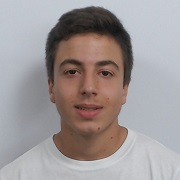
\includegraphics[width=\linewidth]{images/capa/80.jpeg} 
                \centering
                \captionsetup{A89597}
            \endminipage
            \hfill
            \minipage{0.24\textwidth}
                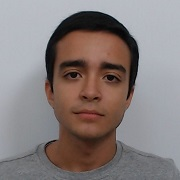
\includegraphics[width=\linewidth]{images/capa/154.jpeg} 
                \centering
                \captionsetup{PG47577}
            \endminipage
            \hfill
            \minipage{0.24\textwidth}
                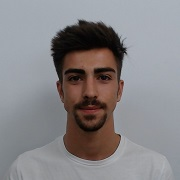
\includegraphics[width=\linewidth]{images/capa/137.jpeg} 
                \centering
                \captionsetup{PG47068}
            \endminipage
            \hfill
            \minipage{0.24\textwidth}
                
\includegraphics[width=\linewidth]{images/capa/152.png} 
                \centering
                \captionsetup{PG47187}
            \endminipage
        \end{figure}

        \vspace{4cm}
        
        11 de janeiro de 2022
            
    \end{center}
\end{titlepage}

\tableofcontents
\thispagestyle{empty}

\setcounter{page}{1}


%-----------------------------------------------------------------%
\clearpage
\section{Introdução}

O presente relatório serve como estrutura de explicação e apresentação da realização do Trabalho Prático no âmbito da unidade curricular de Aplicações e Serviços de Computação em Nuvem. 

O Trabalho Prático terá como objetivo primordial a caracterização, análise, instalação e avaliação da aplicação \textit{Wiki.js}. Além disso, e para alcançar com sucesso a realização deste projeto, serão ainda colocados em prática todos os assuntos e conceitos lecionados nas aulas ao longo do semestre, por forma a garantir a automatização completa de processos de instalação, monitorização e avaliação da aplicação.

Desta forma, o trabalho prático foi dividido em 4 etapas/tarefas principais. Na primeira etapa, iremos abordar qual a arquitectura, padrões de distribuição e componentes da aplicação, fazendo uma descrição das mesmas e passando ainda por perceber operações críticas tomadas de forma a obter um bom desempenho e uma alta disponibilidade da aplicação. Na segunda etapa, iremos explicar quais as ferramentas e abordagens utilizadas de forma a obter a instalação e configuração automática da aplicação, percebendo ainda os motivos para tais escolhas e decisões. Na terceira etapa, iremos apresentar as ferramentas de monitorização e métricas escolhidas, fazendo também uma breve justificação das escolhas tomadas. Por fim, temos a quarta etapa onde iremos explicar quais as ferramentas de avaliação utilizadas no Trabalho Prático, justificando a nossa escolha, apresentando e analisando os resultados provenientes de uma avaliação experimental.

Desta forma, o relatório estará dividido nestas 4 etapas, explicando e apresentando cada uma delas sequencialmente.


%-----------------------------------------------------------------%
\clearpage
\section{Primeira etapa}

Esta etapa do trabalho prático consiste em compreender a arquitetura e os componentes da aplicação \textit{Wiki.js}, bem como identificar os seus padrões de distribuição e os componentes críticos para a sua execução.

\subsection{Descrição da Arquitetura da Aplicação}

O nosso trabalho recai sobre uma arquitetura \textit{Multi-tier}, no qual cada servidor atua como cliente do nível seguinte. Deste modo, concede a escabilidade de diversas finalidades e uma efetivação autónoma. Melhor dizendo, possuímos três VMs, nomeadamente, uma com a tarefa referente à WEB, sendo que no caso do nosso projeto se trata de Wiki.js;  uma segunda relacionada com a parte alusiva à base de dados e, por fim,  a VM a qual denominamos \textit{master}, cujo papel se traduz em criar o \textit{cluster} e geri-lo. Ademais, encarrega-se por obter dados do \textit{Metricbeat} resultante dos \textit{workers} (sendos os mesmos as restantes duas VMs).

\subsection{Identificação dos Padrões de Distribuição e dos componentes da aplicação}

Os componentes principais e críticos desta aplicação são, então, o Wiki.js e a base de dados, Postgres.
Estes são instalados através da execução do \textit{Playbook}.

\subsection{Identificação das Operações Críticas}

Umas das operações críticas identificadas pelo nosso grupo são a instalação do Docker e do Kubernetes, dado que estas ferramentas são necessárias para a criação de um \textit{cluster} e consequente execução da aplicação. Esta operação foi efetuada da seguinte forma:

\begin{itemize}
    \item Primeiramente, é adquirido o repositório do Docker e instalado de seguida. Depois é configurado e reiniciado.
    
    \item De seguida, efetua-se um procedimento semelhante para instalar o Kubernetes.
    
    \item São instaladas, também, umas ferramentas de rede e é desativado o serviço swap.
\end{itemize}

%-----------------------------------------------------------------%
\section{Segunda etapa}

Nesta etapa foi-nos requisitado o uso de ferramentas apropriadas para uma instalação automática e configurável dos diversos componentes da aplicação Wiki.js num ambiente de computação em nuvem, neste caso, na Google Cloud Platform.

\subsection{Identificação das ferramentas e abordagem utilizadas para a instalação e configuração automática da aplicação}

De forma a proceder a uma instalação automática dos componentes da aplicação, decidimos usar o Ansible, pois é uma ferramenta que permite automatizar o \textit{deployment} e escalamento de aplicações de uma maneira eficiente e simplificada.

No caso da aplicação Wiki.js, começamos por criar as VMs necessárias (um nodo \textit{master} e um ou mais nodos \textit{worker}) usando partido da coleção de módulos \textit{Google.Cloud}.

Depois, seguimos para a instalação do Docker e Kubernetes em todos os nodos presentes, de forma a podermos distribuir os diversos componentes da aplicação por vários \textit{containers}.

Após a instalação do Kubernetes, inicializamos o \textit{cluster} no nodo \textit{master} e ligamos os nodos \textit{worker} a este.

Tendo o \textit{cluster} configurado, podemos prosseguir para o \textit{deployment} da aplicação neste. Para tal, decidimos separá-la em duas componentes: a aplicação em si e a sua base de dados. Assim, criamos um nodo no \textit{cluster} para cada uma destas componenetes, permitindo descentralizar a carga da aplicação, distribuindo-a por vários \textit{containers}, obtendo um melhor balanceamento desta.

Tendo em conta a estrutura do nosso \textit{Playbook}, é possível escalar a aplicação de duas formas:

\begin{itemize}
    \item \textbf{Aumentando o número de nodos \textit{worker}}, permitindo ter mais do que uma máquina virtual associada a certa componenta da aplicação.
    \item \textbf{Aumentando o número de \textit{pods} num nodo do \textit{cluster}}, permitindo distribuir a carga dentro deste.
\end{itemize}


%-----------------------------------------------------------------%
\section{Terceira etapa}

Esta etapa consiste em dotar a aplicação instalada de ferramentas de monitorização que permitam observar a aplicação num ambiente de testes e/ou produção.

\subsection{Ferramentas de monitorização e métricas escolhidas}

A monitorização de uma aplicação pode ser dividida em quatro etapas: observação, recolha, análise e apresentação. Decidimos usar a \textit{Elastic Stack}, pois disponibiliza serviços para esta quatro etapas (\textit{Metricbeats}, \textit{Logstash}, \textit{Elasticsearch} e \textit{Kibana}, repetivamente).

Em relação ao \textit{Metricbeats}, este corre nos nodos \textit{worker}, obtendo informações dos eventos diretamente do sistema, observando os seus recursos. Este serviço tem, também, a capacidade de normalizar os dados e enviá-los para o \textit{Elasticsearch}. Este irá analisar e processar a informação, preparando-a para ser apresentada. A fase de apresentação é da responsabilidade do \textit{Kibana}, usando partido da indexação feita anteriormente.


%-----------------------------------------------------------------%
\section{Quarta etapa}

Nesta etapa foi-nos requisitado que considerássemos ferramentas de avaliação para a aplicação.

\subsection{Ferramentas de avaliação e testes desenvolvidos}

De forma a avaliar o desempenho da aplicação no nosso \textit{cluster}, decidimos usar o JMeter para simular o uso da nossa aplicação por parte de vários utilizadores simultâneos e analisamos os dados usando as suas funcionalidades, como também as do Kibana.

Em relação aos testes desenvolvidos, corremos a ferramenta de HTTP Request do JMeter, para 1, 10 e 100 threads, durante alguns segundos.

\subsection{Apresentação e análise dos resultados da avaliação experimental}

Pela análise das figuras seguintes, podemos concluir que o nodo que contém a aplicação Wiki.js sofre no desempenho, com o aumento de pedidos simultâneos. Isto deve-se, principalmente, ao aumento do uso do CPU. Em relação à memória, esta mantém-se estável. Já o nodo referente à base de dados não sofre quebras no desempenho, com o aumento do número de pedidos em simultâneo.

\begin{figure}[H]
    \centering
    \frame{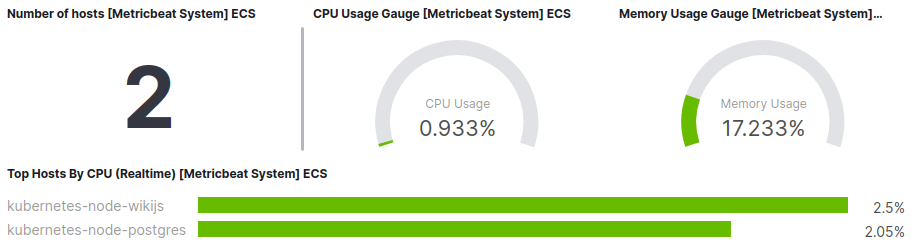
\includegraphics[width=\textwidth]{images/testes/1_thread_overall.png}}
    \caption {Resultados Kibana - 1 Thread}
\end{figure}

\begin{figure}[H]
    \centering
    \frame{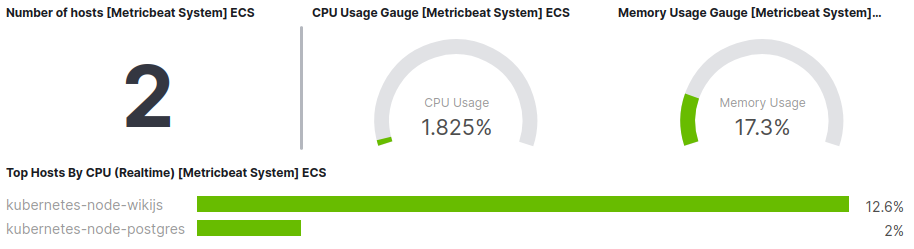
\includegraphics[width=\textwidth]{images/testes/10_thread_overall.png}}
    \caption {Resultados Kibana - 10 Threads}
\end{figure}

\begin{figure}[H]
    \centering
    \frame{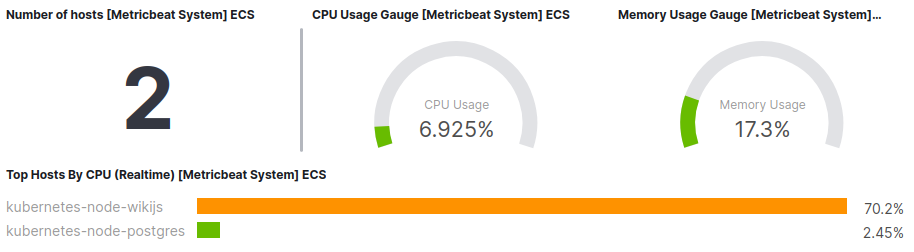
\includegraphics[width=\textwidth]{images/testes/100_thread_overall.png}}
    \caption {Resultados Kibana - 100 Threads}
\end{figure}


\begin{figure}[H]
    \centering
    \frame{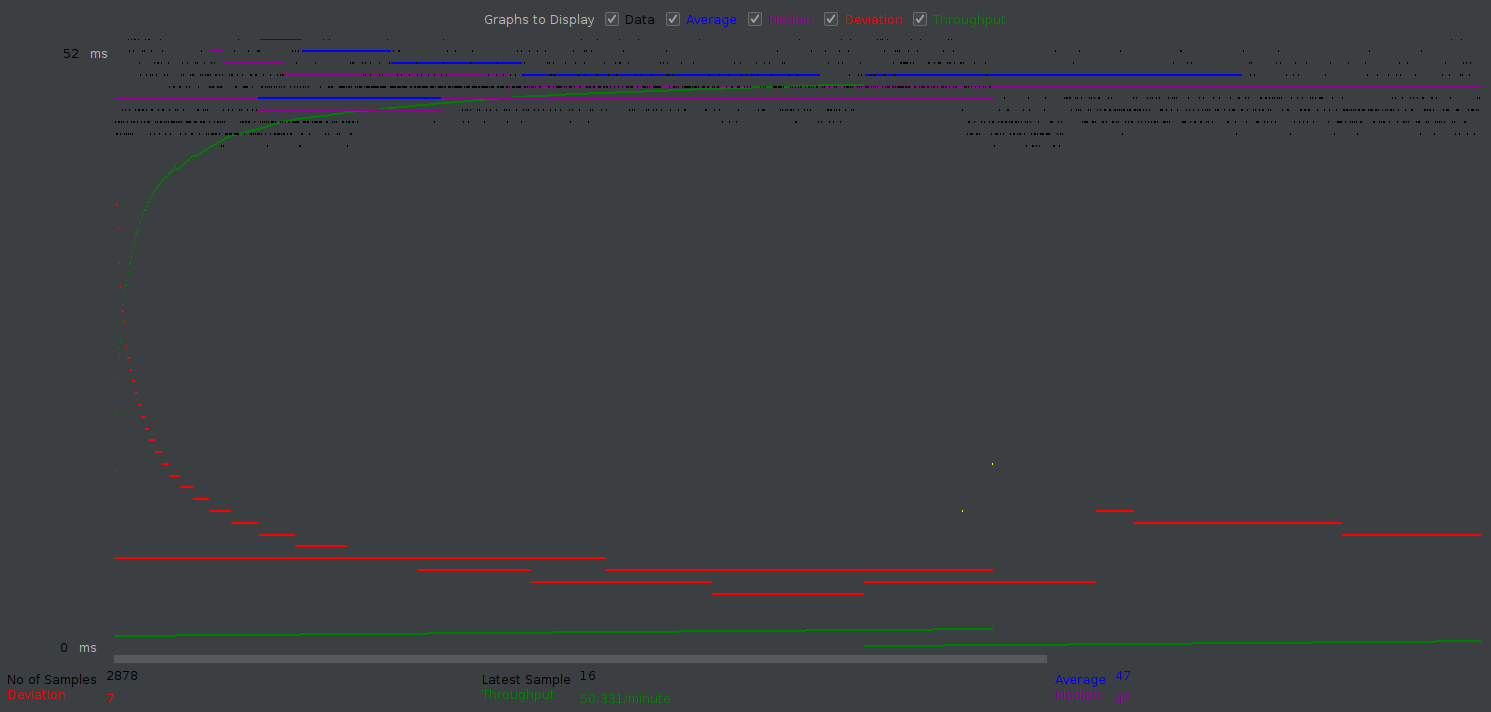
\includegraphics[width=\textwidth]{images/testes/1_thread_graph.png}}
    \caption {Gráfico JMeter - 1 Thread}
\end{figure}

\begin{figure}[H]
    \centering
    \frame{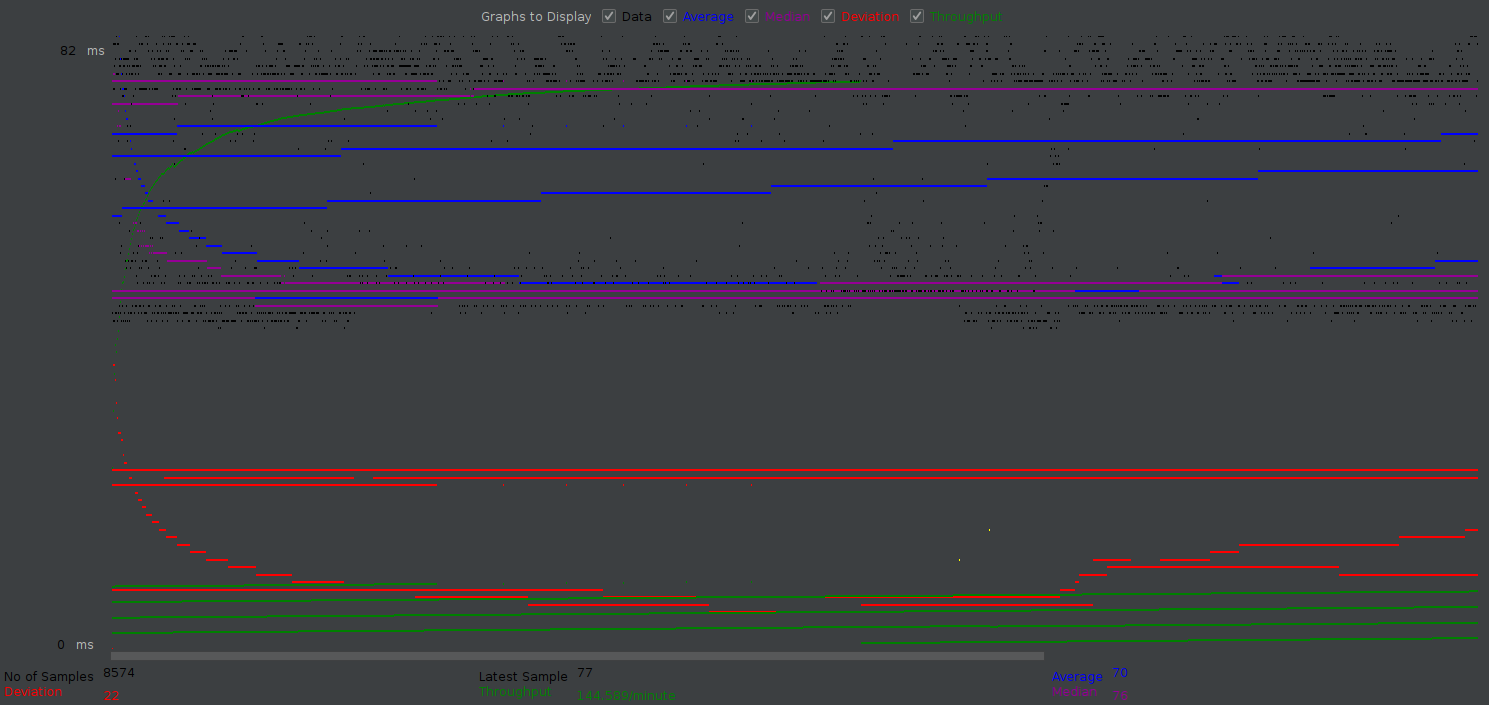
\includegraphics[width=\textwidth]{images/testes/10_thread_graph.png}}
    \caption {Gráfico JMeter - 10 Threads}
\end{figure}

\begin{figure}[H]
    \centering
    \frame{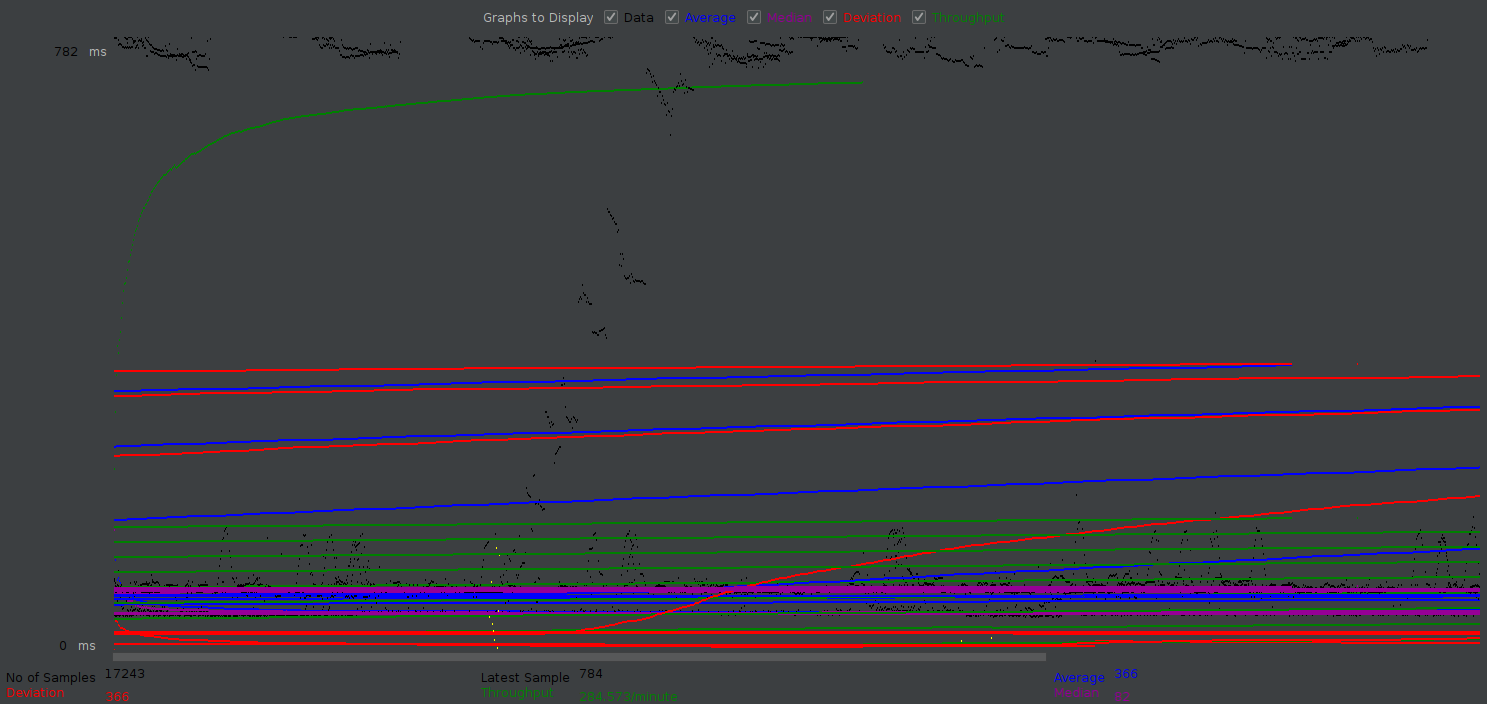
\includegraphics[width=\textwidth]{images/testes/100_thread_graph.png}}
    \caption {Gráfico JMeter - 100 Threads}
\end{figure}


\begin{figure}[H]
    \centering
    \frame{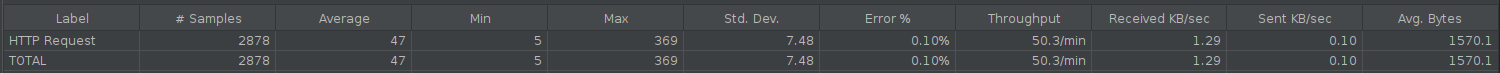
\includegraphics[width=\textwidth]{images/testes/1_thread_summary.png}}
    \caption {Resumo JMeter - 1 Thread}
\end{figure}

\begin{figure}[H]
    \centering
    \frame{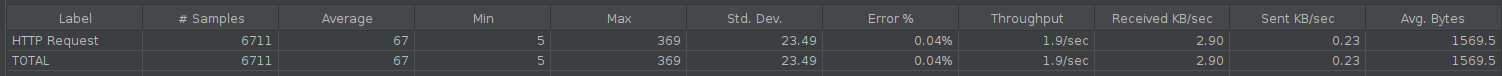
\includegraphics[width=\textwidth]{images/testes/10_thread_summary.png}}
    \caption {Resumo JMeter - 10 Threads}
\end{figure}

\begin{figure}[H]
    \centering
    \frame{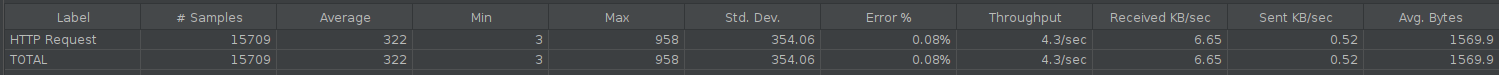
\includegraphics[width=\textwidth]{images/testes/100_thread_summary.png}}
    \caption {Resumo JMeter - 100 Threads}
\end{figure}


%-----------------------------------------------------------------%
\clearpage
\section{Conclusão}

Assim, e compreendida a aposta inicialmente dada que consistia na caracterização, análise, instalação e avaliação da aplicação \textit{Wiki.js}, foram postas as "mãos na massa". Desta forma, e utilizando técnicas e conceitos aprendidos ao longo do semestre nas aulas práticas e teóricas, achamos ter realizado com sucesso a componente prática que nos foi fornecida. Além disso, conseguimos também consolidar todos estes conhecimentos obtidos na unidade curricular de Aplicações e Serviços de Computação em Nuvem, obtendo o melhor dos dois mundos.

Ademais, podemos constatar que os objectivos foram de uma forma geral alcançados, deixando ainda uma ideia na equipa de realização e cumprimento face às escolhas e decisões tomadas ao longo da realização da concepção do projeto. No entanto, achamos que poderíamos ter melhorado em dois pormenores em específico. Um deles foi que não conseguimos utilizar com sucesso \textit{secrets}, não conseguindo dessa forma haver a encriptação que nós desejávamos. O outro pormenor foi o de não termos conseguido deixar correr o \textit{Playbook} quando as instâncias já existem, tornando-se assim a única parte idempotente na totalidade do projeto (todas as outras \textit{Tasks} podem ser corridas mesmo que já tenham sido corridas antes). Ainda assim, a equipa detém orgulho e encontra-se feliz com o projeto realizado e a concepção conseguida.

Concluindo, é importante novamente realçar a importância do projeto face à consolidação obtida dos conceitos e técnicas dados durante todo o semestre, ficando a certeza de que mais tarde, no mundo do trabalho, os poderemos aplicar correta e devidamente quando assim for necessário.

\end{document}
